\chapter{Weight Estimation}
\section{Introduction}
To develop UDAAN - a lightweight, energy efficient, inflatable drone capable of vertical Take off, Stand By and Landing, which can deliver payloads and is self rechargeable.
Drones allows for a wide variety of missions, however with the weight of the sensors increasing, the drones able to carry such payloads are cumbersome and difficult to transport.That is why we are trying to develop India's first inflatable drone.The drone has inflatable structure, is at the same time will be easy to transport and rugged because of the flexible structure. Moreover, the drone would be waterproof and can land and take-off on water surface because of compressed Helium gas used in the inflatable structure. 


\section{Novelty Features}

\subsection{Fast}

The UDAAN will unfold in a few seconds and can be operated by a single person.

\subsection{Compact}

The UDAAN will be easily transportable thanks to its compact and foldable inflatable structure

\begin{figure}[h!]
\centering
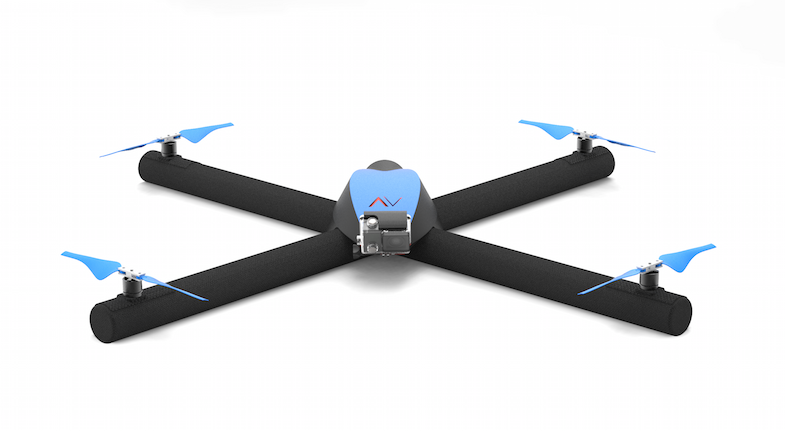
\includegraphics[width=.8\textwidth]{drone.png} 
\caption{\label{fig:drone}Inflatable drone}
\end{figure}

\subsection{Amphibious}

The UDAAN is waterproof, therefore deployable under heavy rain or even on water.

\subsection{Payload and Surveillance}

UDAAN is capable of carrying a Payload and hence can be utilised for delivery of items via e-commerce channel.


\subsection{Self Rechargeable}

UDAAN would be equipped with self rechargeable capabilities.We are trying to develop and incorporate a mechanism to recharge the battery using renewable energy sources. 




\clearpage
\section{Mission Profile} .

\begin{figure}[h!]
\centering
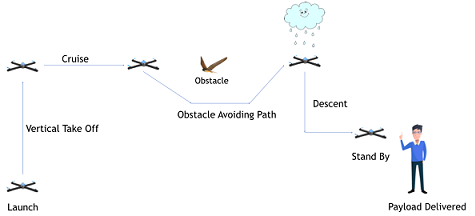
\includegraphics[width=1.1\textwidth]{mission_profile.png} 
\caption{\label{fig:mission_profile}Mission Profile}
\end{figure}


\section{Estimated Data}

\subsection{Dimensions}

Available Payload : Camera, Parcel

Folded : 300x300x150 mm

Unfolded : 800x800x150 mm

Endurance : up to 60 min

\subsection{Common Characteristics}

Waterproof

Wind resistance : 37 kmph

Unfolding time : ‹60s

Folding time : ‹60s

\subsection{Weight Estimate}
\begin{table}[h!]
 \begin{center}
 \begin{tabular}{|c| c |c |c|} 
 \hline
 Components & Weight(grams) & Quantity & Total Weight(grams) \\ [0.5ex] 
 \hline
 Propeller & 5 & 4 & 5*4=20 \\ 
 \hline
 Motor & 20 & 4 & 20*4=80 \\
 \hline
 Flight Control Board & 50  & 1 & 50*1=50 \\
 \hline
 Electronic speed controller & 75 & 4 & 75*4=300 \\ 
 \hline
 Base weight & 100 & 1 & 100*1=100 \\ 
 \hline
 Camera weight & 120 & 1 & 120*1=120 \\ 
 \hline
 Battery & 200 & 1 & 200*1=200 \\ 
 \hline
\end{tabular}
\caption{\label{table:weight_estimatio}First Weight Estimation}
\end{center}

\end{table}
Total weight = 20+80+50+300+100+120+200=870 grams

Data given in the table are initial guesses and actual weight might vary from this approximation.


